\chapter[Ontological Structures of Persuasive Game Design in CL Scenarios]{Ontological Structures of Persuasive Game Design in Collaborative Learning Scenarios}
\label{chapter:ontogacles-2}

In the previous chapter, ontological structures have been formalized in the ontology OntoGaCLeS to represent the personalization of gamification in CL scenarios based on player type models. These ontological structures have been proposed to support the definition of player roles and the selection of game elements for each participant in a CL scenario. However, to deal with the motivation problem caused by the scripted collaboration, it is also necessary to provide support for the design of CL gameplay. This design consists into setting up the selected game elements to persuade the participants to follow the interactions defined by a CSCL script in which the CL process of CL scenario has been based. To accomplish this, gamification as Persuasive Game Design (PGD) should be linked to the design of CL process.

This chapter present the ontological structures proposed by the author of this PhD thesis dissertation to represent the connection between PGD and the design of CL process in CL scenarios. This connection intends to solve the context-dependency of gamification related to the non-game context and target behaviors being gamified with the purpose to deal with the motivation problem caused by the scripted collaboration. Thus, the first section (\autoref{sec:modeling-game-non-game-worlds}) presents a nested-structure proposed to identify things that belong to the game world and non-game world. Having this clearly separation, the formalization of PGD as ontological structures is presented in \autoref{sec:modeling-persuasive-game-design-gamification-cl-scenarios}. Then, the ontological structures proposed to represent the CL gameplay based on PGD are presented in \autoref{sec:modeling-cl-gameplay-persuasive-game-design}. To demonstrate the usefulness of these ontological structures, \autoref{sec:formalizing-ontological-model-apply-gamification-persuasive-technology} shows the formalization of an ontological model to apply gamification as persuasive technology in Cognitive Apprenticeship scenarios. Finally, \autoref{sec:ontogacles2-concluding-remarks} presents the concluding remarks of this chapter.
 
Part of the work described in this chapter was published by the author of this PhD thesis dissertation in the scientific articles:

\begin{itemize}
\item
\aspas{\emph{Steps Towards the Gamification of Collaborative Learning Scenarios Supported by Ontologies}} published in the 17\textsuperscript{th} International Conference on Artificial Intelligence in Education, AIED 2015, held in Madrid, Spain \cite{ChallcoMizoguchiBittencourtIsotani2015a}.

\item
\aspas{\emph{An Ontological Model to Apply Gamification as Persuasive Technology in Collaborative Learning Scenarios}} published in the 26\textsuperscript{th} Brazilian Symposium on Computer in Education, SBIE 2015, held in Maceió, AL, Brazil \cite{ChallcoAndradeOliveiraMizoguchiIsotani2015}.

\item
\aspas{\emph{Gamification of Collaborative Learning Scenarios: Structuring Persuasive Strategies Using Game Elements and Ontologies}} published in the 1\textsuperscript{st} International Workshop on Social Computing in Digital Education, SocialEdu 2015, held in Stanford, CA, USA \cite{ChallcoMizoguchiBittencourtIsotani2015}.

\item
\aspas{\emph{An Ontology Framework to Apply Gamification in CSCL Scenarios as Persuasive Technology}} published as Volume 24, Issue 2, in the Brazilian Journal of Computers in Education - RBIE, 2016 \cite{ChallcoMizoguchiIsotani2016}.
\end{itemize}

%%%%%%%%%%%%%%%%%%%%%%%%%%%%%%%%%%%%%%%%%%%%%%%%%%
\section{Modeling Game and Non-game Worlds}
\label{sec:modeling-game-non-game-worlds}

One of the main difficulties to formally represent the gamification in a computer understandable manner is the lack of a clearly separation between game world and non-game world. As was mentioned at the \autoref{chapter:general-background}, a game is a problem-solving activity approached with playful attitude\footnote{A gameful attitude is defined here as a playful attitude in which the intrinsic motivation is a necessary condition to achieve this attitude, but the immersion and enjoyment are desirable conditions}\cite{Schell2008}, and a non-game context is being gamified with the intention to make it more game-like \cite{Werbach2014}. Therefore, to make the interactions defined by a CSCL script more game-liking in a gamified CL scenario, the gamification process consists into add game elements in the environment in which the actions of participants will take place, and to define how these game elements will interact with the participants during the CL process. In this gamification process, gamification models and/or frameworks are used to explain the game design process using a theoretical foundation in game design models. The game elements and their interaction with the students produce and/or induce changes in the psychological state of participants, and these changes are theoretically justified through theories/models of motivation and human behavior.

Based on this description of gamification process, a nested-structure sees adequate to enable a systematic separation of things between  the game world and non-game world.

the interactions between the participants and game elements are formalized as events, 

 \autoref{fig:nested-structure-game-nongame-worlds} shows this model in which the nested-structure classify the events in two types: the non-game events and the game events. The non-game events describe the activities/actions in the CL process that have the potential to be gamified, and the game events describe the activities/action of game elements to make the activities/actions described in the non-game events more game-like. The theoretical justification in this nested-structure for the gamification process are given as follows: \emph{gamification models and/or frameworks} explain the \emph{game design process} used to introduce and to define \emph{game events} whereby the non-game situation becomes more game-like; the reasons why these \emph{game events} had been introduced in the non-game situation is explained by \emph{game design models}; and the changes produced and/or induced by the game events are explained by \emph{theories/models of motivation and human behavior}. 

\begin{figure}[!htb]
 \caption{Nested structure of non-game world, game world and gamification world}
 \label{fig:nested-structure-game-nongame-worlds}
 \centering
 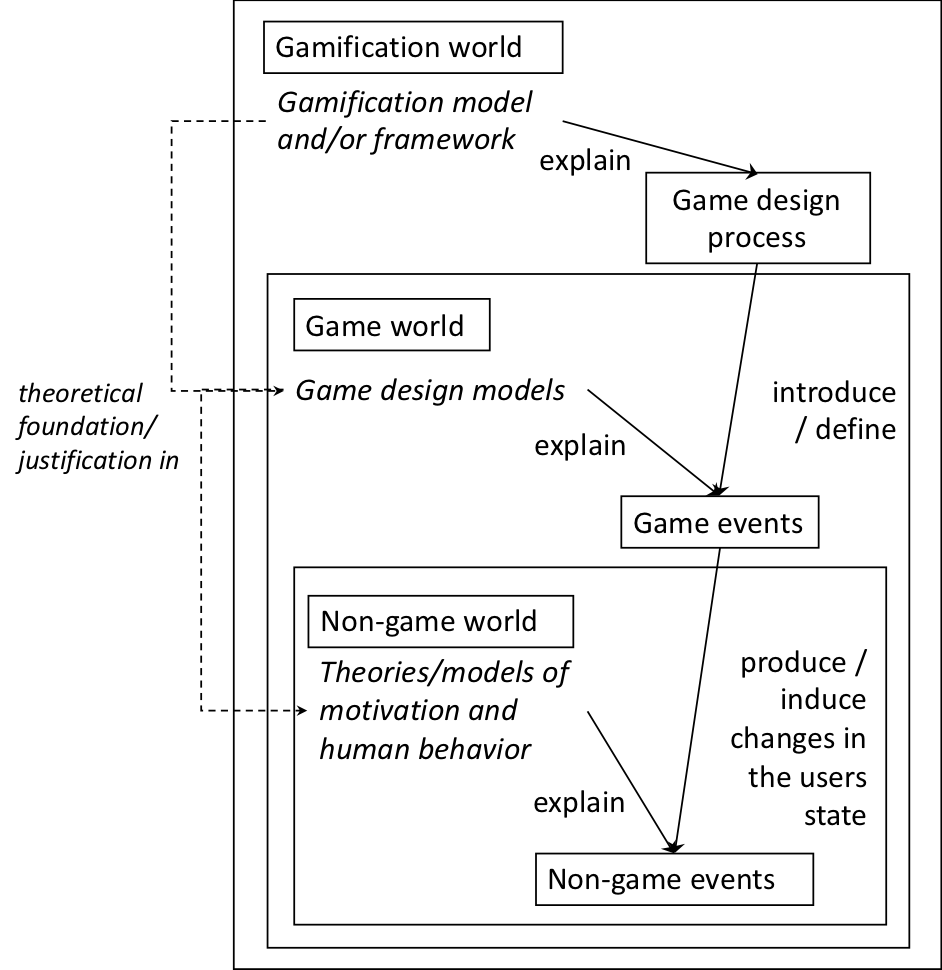
\includegraphics[width=0.55\textwidth]{images/chap-ontogacles2/nested-structure-game-nongame-worlds.png}
 \fautor
\end{figure}

Employing the nested-structure of non-game world, game world and gamification world (\autoref{fig:nested-structure-game-nongame-worlds}), the concepts in the ontology OntoGaCLeS related to the game events and non-game events have been classified in the \aspas{\emph{is-a}} hierarchy structure of class shown in \autoref{fig:is-a-hierarchy-structure-of-classes}. This structure categorizes any concept of ontology as a sub-type of classes: \emph{Gamification world}, \emph{Game world}, Non-game world, Common world, and Theory/Model. The classes defined under the categories of common, non-game, game and gamification worlds are concepts for things in their respective worlds, and the concepts formalized as sub-type of \emph{Theory/Model} define the theoretical foundation and justification of gamification, and game design.

\begin{figure}[!htb]
 \caption{\aspas{\emph{is-a}} hierarchy structure of classes to represent concepts in the ontology OntoGaCLeS}
 \label{fig:is-a-hierarchy-structure-of-classes}
 \centering
 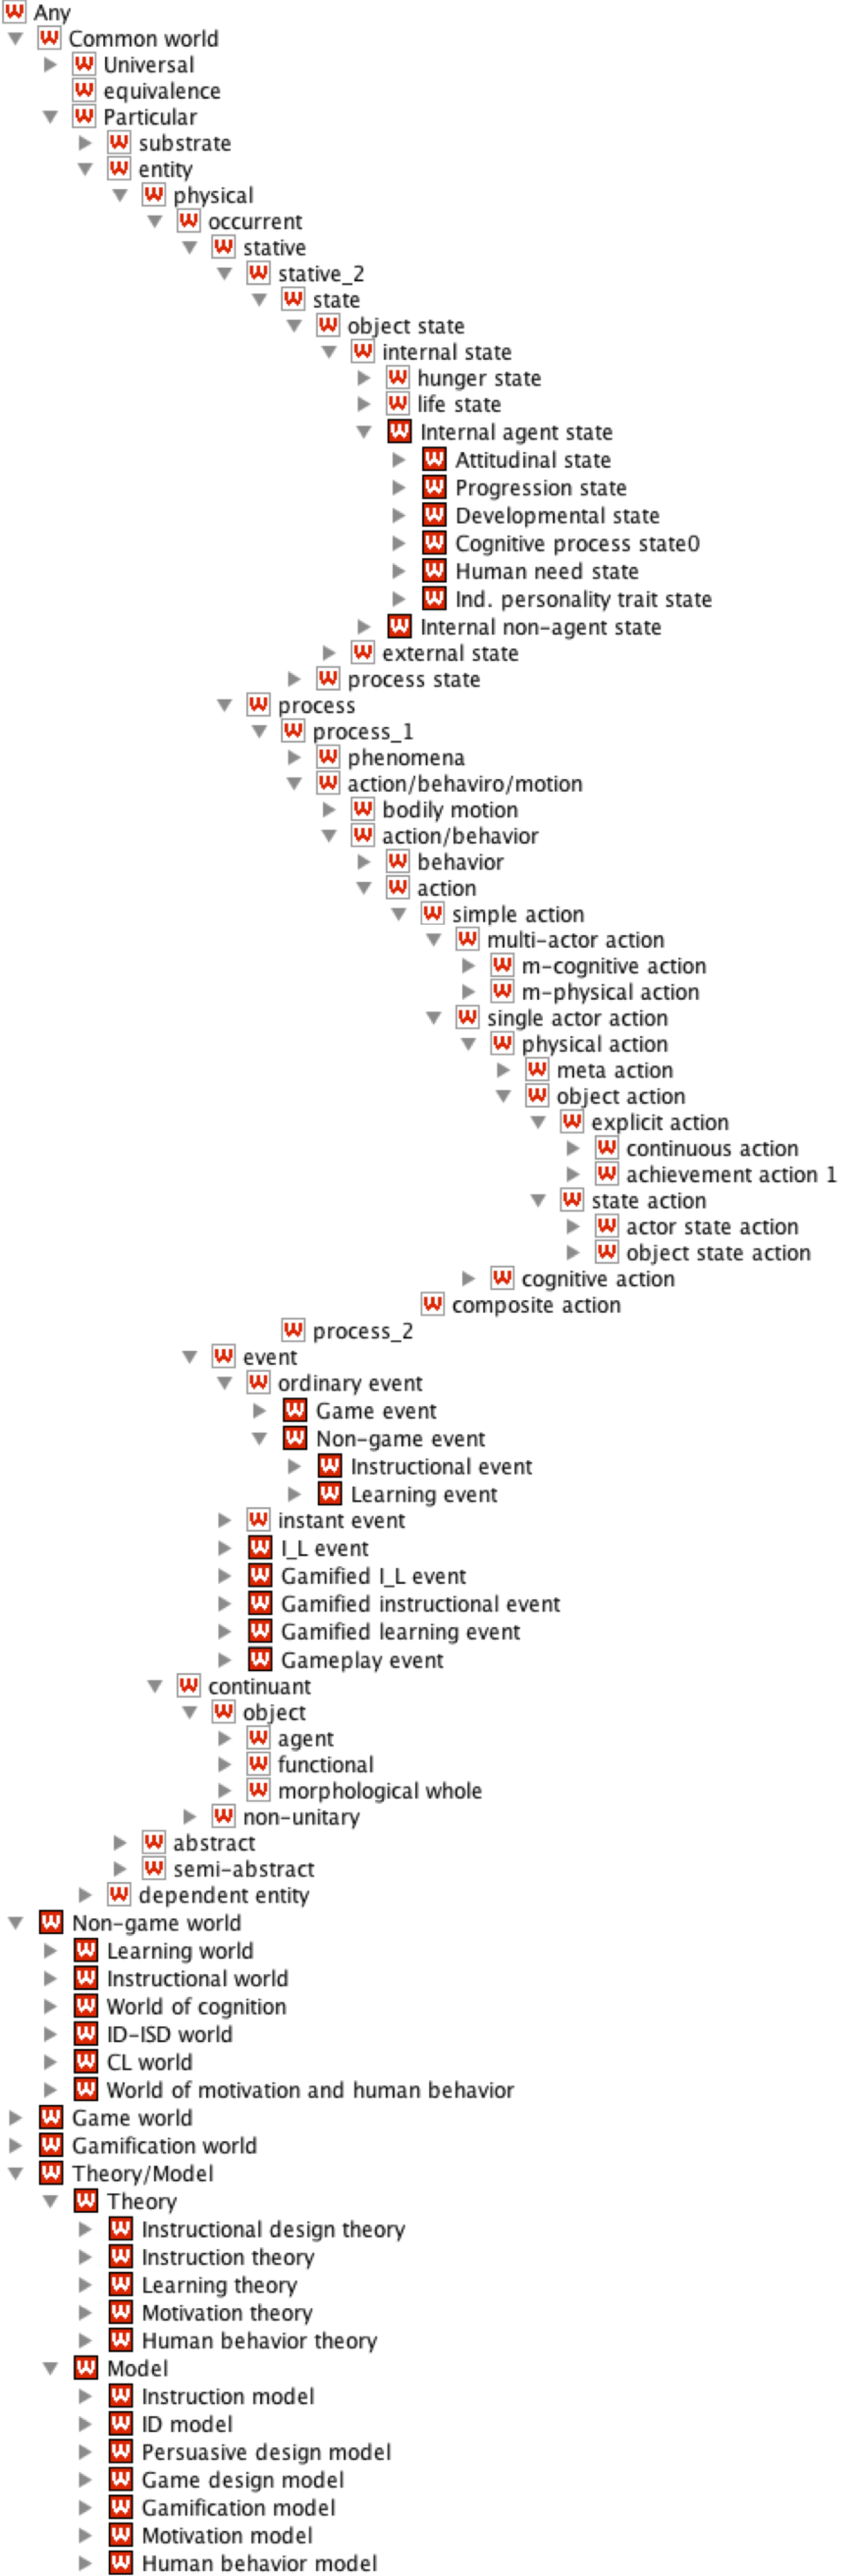
\includegraphics[width=0.45\textwidth]{images/chap-ontogacles2/is-a-hierarchy-structure-of-classes.png}
 \fautor
\end{figure}
\newpage

\emph{Gamification world} is the class of all things that depend of the gamification world to exist. In this sense, a concept is formalized as sub-type of \emph{Gamification world} whether it represents something that needs of gamification world to be described. For instance, the \emph{Gamification goal/purpose} is a concept formalized as sub-type of Gamification world to describe the goals and/or purposes of a gamification model and/or framework (e.g. \emph{avoiding dropout}, \emph{reducing weariness}). The basic concepts defined as sub-types of \emph{Gamification world} for the gamification of CL scenarios are: \emph{Gamified CL session}, \emph{Motivational strategy}  (\emph{Y<=I-mot goal}) by gamification, \emph{Player role}, and \emph{Individual gameplay strategy} (\emph{I-gameplay strategy}).

\emph{Game world} is the class of all things that depend of the game world to exist. Concepts formalized as sub-types of \emph{Game world} require only elements defined in the games to be described. The basic concept defined as sub-types of \emph{Game world} to gamify CL scenarios is: \emph{Game element}. \emph{Non-game world} is the class of all things that does not need concepts from the \emph{Gamification world} or \emph{Game world} to exist. The non-game world is divided in the sub-types: \emph{Learning world}, \emph{Instructional world}, \emph{World of cognition}, \emph{ID-ISD world}, \emph{CL world}, and \emph{World of motivation and human behavior}. Basic concepts defined as one of these world only need things from its respectively world to exist. Thus, for instance, the concepts formalized as sub-type of \emph{World of motivation and human behavior} represent things that only need elements from motivation and human behavior to exist, so that the basic concepts related to the gamification of CL scenarios formalized as sub-types of \emph{World of motivation and human behavior} are: Individual motivational goal (\emph{I-mot goal}), \emph{Motivation stage}, and \emph{Human need stage}.

\emph{Common world} is the class of anything used to represent things that require concepts of other worlds to be formalized. These concepts are common to the other worlds, and they have been taxonomically classified taking as base the classification defined in the upper-level ontology \textbf{YAMATO} – \emph{\textbf{Y}et \textbf{A}nother \textbf{M}ore \textbf{A}dvanced \textbf{T}op-level \textbf{O}ntology} \cite{Mizoguchi2010}. The basic concepts in the \emph{Common world} to represent persuasive game design are the concepts of: (i) \emph{action}, (ii) \emph{entity} (e.g. \emph{object}, \emph{agent}), (iii) \emph{state}, and (iv) \emph{event}. These concepts, their sub-types, and their ontological structures have been formalized following the formalization proposed by Galton and Mizoguchi in the article \aspas{\emph{The Water Falls but the Waterfall Does Not Fall: New Perspectives on Objects, Processes and Events}} \cite{GaltonMizoguchi2009}. According to these definitions, there is a mutual dependency between processes and entities whereby no one process (\emph{action}) can exist without an entity (\emph{agent} or \emph{object}) to enact it, and an entity is what it is as consequence of its processes. Therefore, an entity has properties knows as \emph{states} that change over time when processes are enacted by the object. An \emph{event} is then defined as integration of entities, actions, and states in a particular context to describe a fixed chunk of any process in which the participants of process are the agents and objects.

\begin{figure}[!htb]
 \caption{Ontological structures to represent events}
 \label{fig:ontological-structures-event}
 \centering
 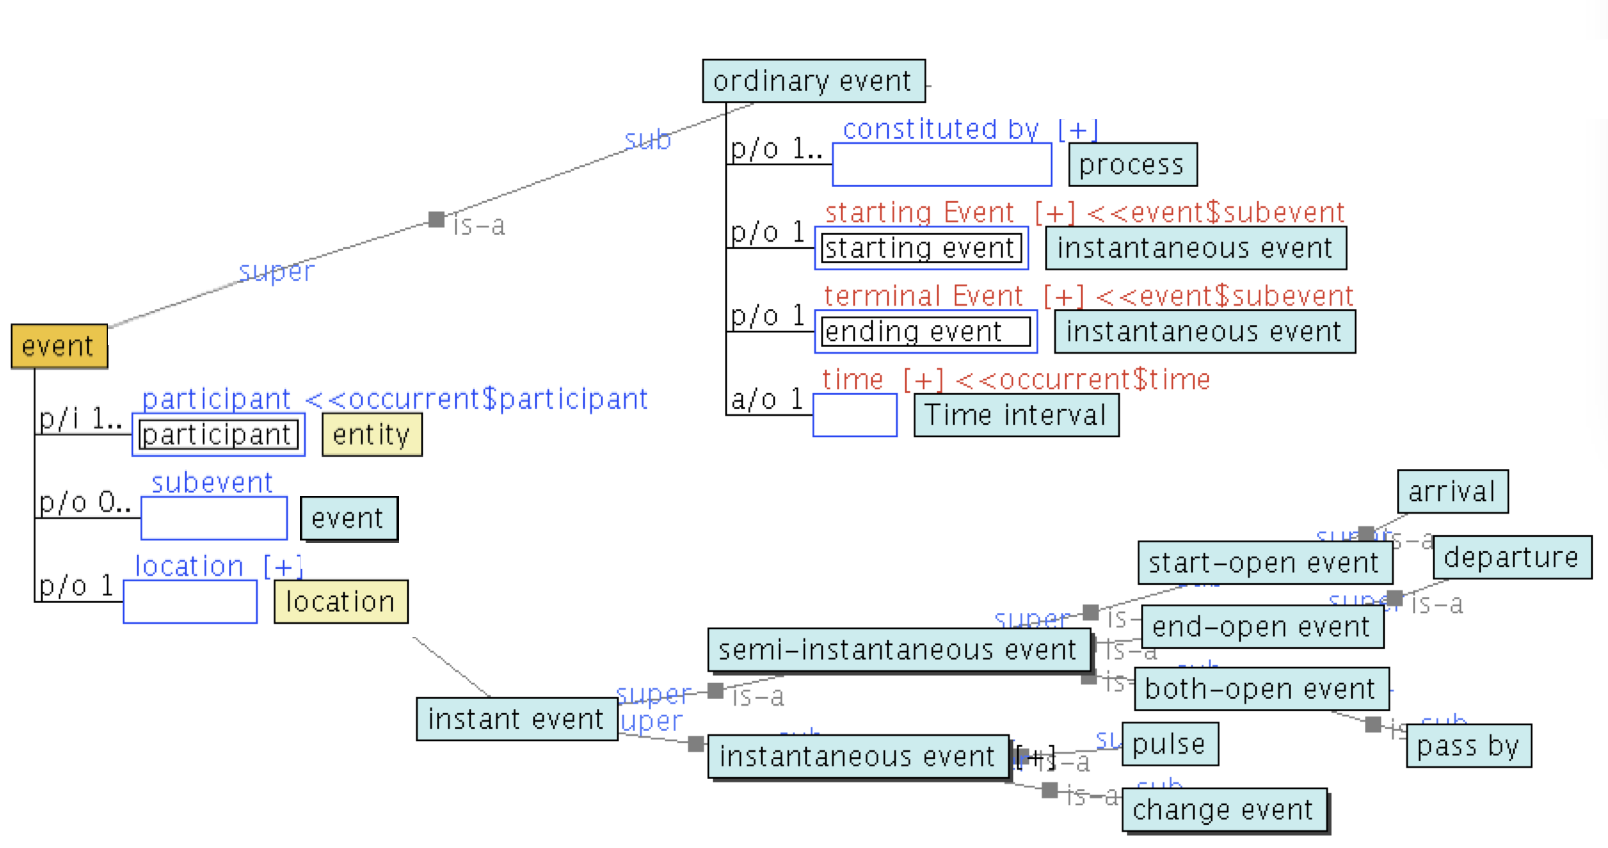
\includegraphics[width=1\textwidth]{images/chap-ontogacles2/ontological-structures-event.png}
 \fautor
\end{figure}

\autoref{fig:ontological-structures-event} shows the formalization of events as ontological structures in the ontology OntoGaCLeS. As it shown in this formalization, the class event is classified in \emph{ordinal event} and \emph{instant event} in which the ordinal event is constituted by a process (e.g. \emph{action}, \emph{behavior}), the participants in the events are entities, and the ordinal event has instantaneous events as starting and ending event to delimit the chunk of processes that compose the event. Finally, the \emph{ordinal event} is classified in \emph{Game event} and \emph{Non-game event} as shown in the \aspas{\emph{is-a}} hierarchy of classes (\autoref{fig:is-a-hierarchy-structure-of-classes}). The composed events in the \aspas{\emph{is-a}} hierarchy structure of classes are defined as subtype of \emph{event}, and they are: \emph{I\_L event}, \emph{Gameplay event}, \emph{Gamified Instructional event}, \emph{Gamified Learning event}, and \emph{Gamified I\_L event}.

%%%%%%%%%%%%%%%%%%%%%%%%%%%%%%%%%%%%%%%%%%%%%%%%%%
\section[Modeling Persuasive Game Design for CL Scenarios as Ontological Structures]{Modeling Persuasive Game Design for Collaborative Learning Scenarios as Ontological Structures}
\label{sec:modeling-persuasive-game-design-gamification-cl-scenarios}

\emph{Persuasive Game Design} (PGD) is defined by the author of this PhD thesis dissertation as \aspas{\emph{the game design for the purpose to change peoples’ attitudes and behaviors through persuasion and social influence without using coercion and/or deception}.} In this sense, to represent the PGD as ontological structures, it is necessary an ontology-based formalization of \emph{game design} because PGD is conceptualized as a game design that is embedded in a persuasive design.

As was explained in the previous section, the game design models are used to define the game events whereby the changes in the users’ states are produced or induced in a non-game events, and these changes are explained by theories/models of motivation a human behavior. Therefore, the game design consist into establish the relation between non-game event and game event based theoretical justification extracted from game design models and theories of motivation and human behavior. This game design when the theoretical justification is extracted from PGD models is the PGD, and it has been formalized in the ontology OntoGaCLeS by means of two ontological structures. The former ontological structure is a descriptive form, known as \emph{persuasive gameplay event}, and it is detailed in \autoref{subsec:persuasive-gameplay-event}. The latter ontological structure is a prescriptive form, known as \emph{WAY-knowledge of PGD}, and it is detailed in \autoref{subsec:way-knowledge-of-persuasive-game-design}.

Employing the ontological structures to represent PGD, the concept of \aspas{\emph{Persuasive Game Design CL Scenario Model}} has been proposed to represent the knowledge of how to apply PGD in the CL process of a CL scenario. This model has the purpose to represent the knowledge about how to persuade the learners to follow the interactions defined by a CSCL script. The formalization of this model as ontological structures is presented in \autoref{subsec:persuasive-game-design-cl-scenario-model}.

\subsection{Persuasive Gameplay Event}
\label{subsec:persuasive-gameplay-event}

The relation between game events and non-game events is explicitly represented in the ontology OntoGaCLeS under the concept of \emph{Gameplay event}. This concept describes, in an explicit way, what happens in the non-game world and the game world when a user performs the processes (actions) defined in the non-game event.



A persuasive gameplay event is a descriptive and explicit description of the relation between game events and a non-game event in which the doer of the non-game event has been persuaded and/or social influenced by the game events.

the gameplay event defines the interactions between the game elements and the participants of non-game process. 



 Thus, the persuasive gameplay event is formalized through the ontological structures shown in \autoref{fig:ontological-structures-persuasive-gameplay-events}, where the \emph{Gameplay event} (at the top of figure) represents any interaction that would occur between the participants and game elements. In the gameplay event, the \emph{Game event} describes actions performed by an \emph{agent} that becomes \emph{Game agent}, an \emph{action} of this agent becomes \emph{Game action}, the \emph{participant} who interacts with the game agent becomes \emph{Player}, and if there is an object produced as consequence of \emph{Game action}, it becomes a \emph{Game component}. Employing this formalization, let us to identify the elements for a gameplay event that represents the interaction of \aspas{\emph{a user obtaining points by making a comment},} such gameplay (shown at the top of \autoref{fig:ontological-structures-example-persuasive-gameplay-events}) is defined as a game event \aspas{\emph{Give points event}} in which the \emph{Point-system} becomes a \emph{Game agent} that performs the \emph{Game action} of \emph{Give points}, and the \emph{Points} given by this system becomes a \emph{Game component}. The \emph{Non-game event} in this gameplay event is \emph{Comment event} in which the action performed by the participant is \emph{Comment}.

\begin{figure}[!htb]
 \caption{Ontological structures to represent events}
 \label{fig:ontological-structures-persuasive-gameplay-events}
 \centering
 %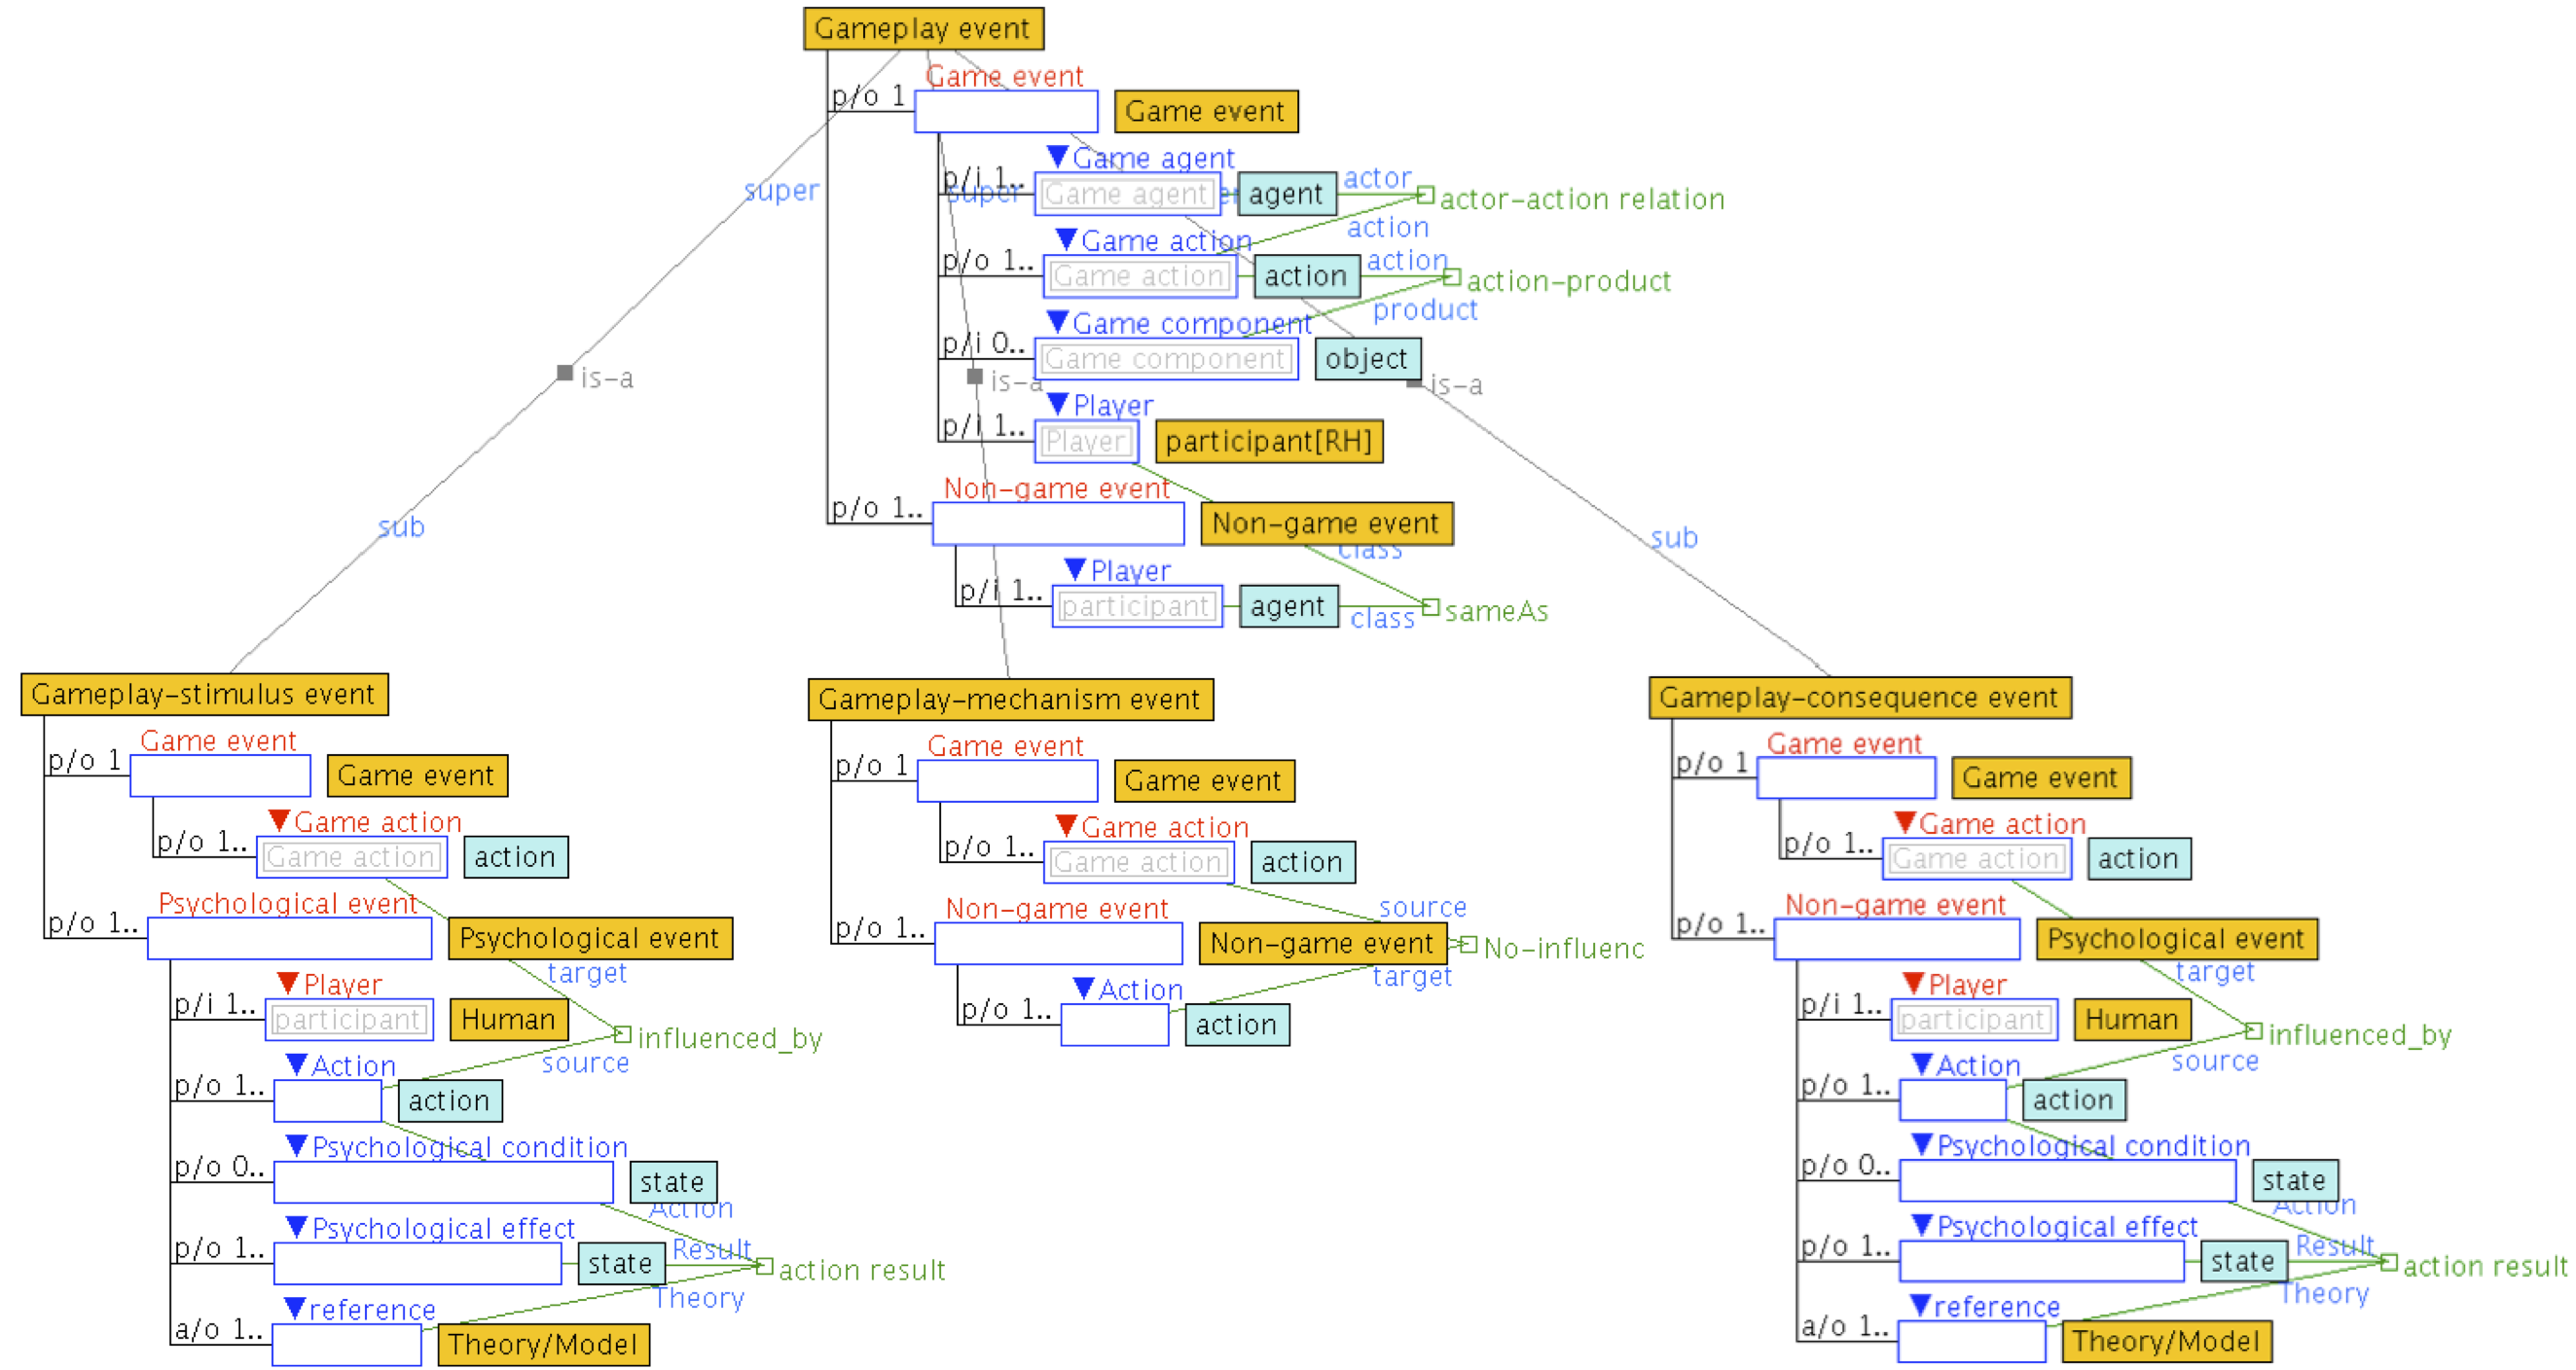
\includegraphics[width=1\textwidth]{images/chap-ontogacles2/ontological-structures-persuasive-gameplay-events.png}
 \fautor
\end{figure}

According to the rules defined in the system, the interaction between the participants and game elements produces changes in the system communicated to the participants. These changes could influence 



\begin{figure}[!htb]
 \caption{Ontological structures to represent events}
 \label{fig:ontological-structures-example-persuasive-gameplay-events}
 \centering
% 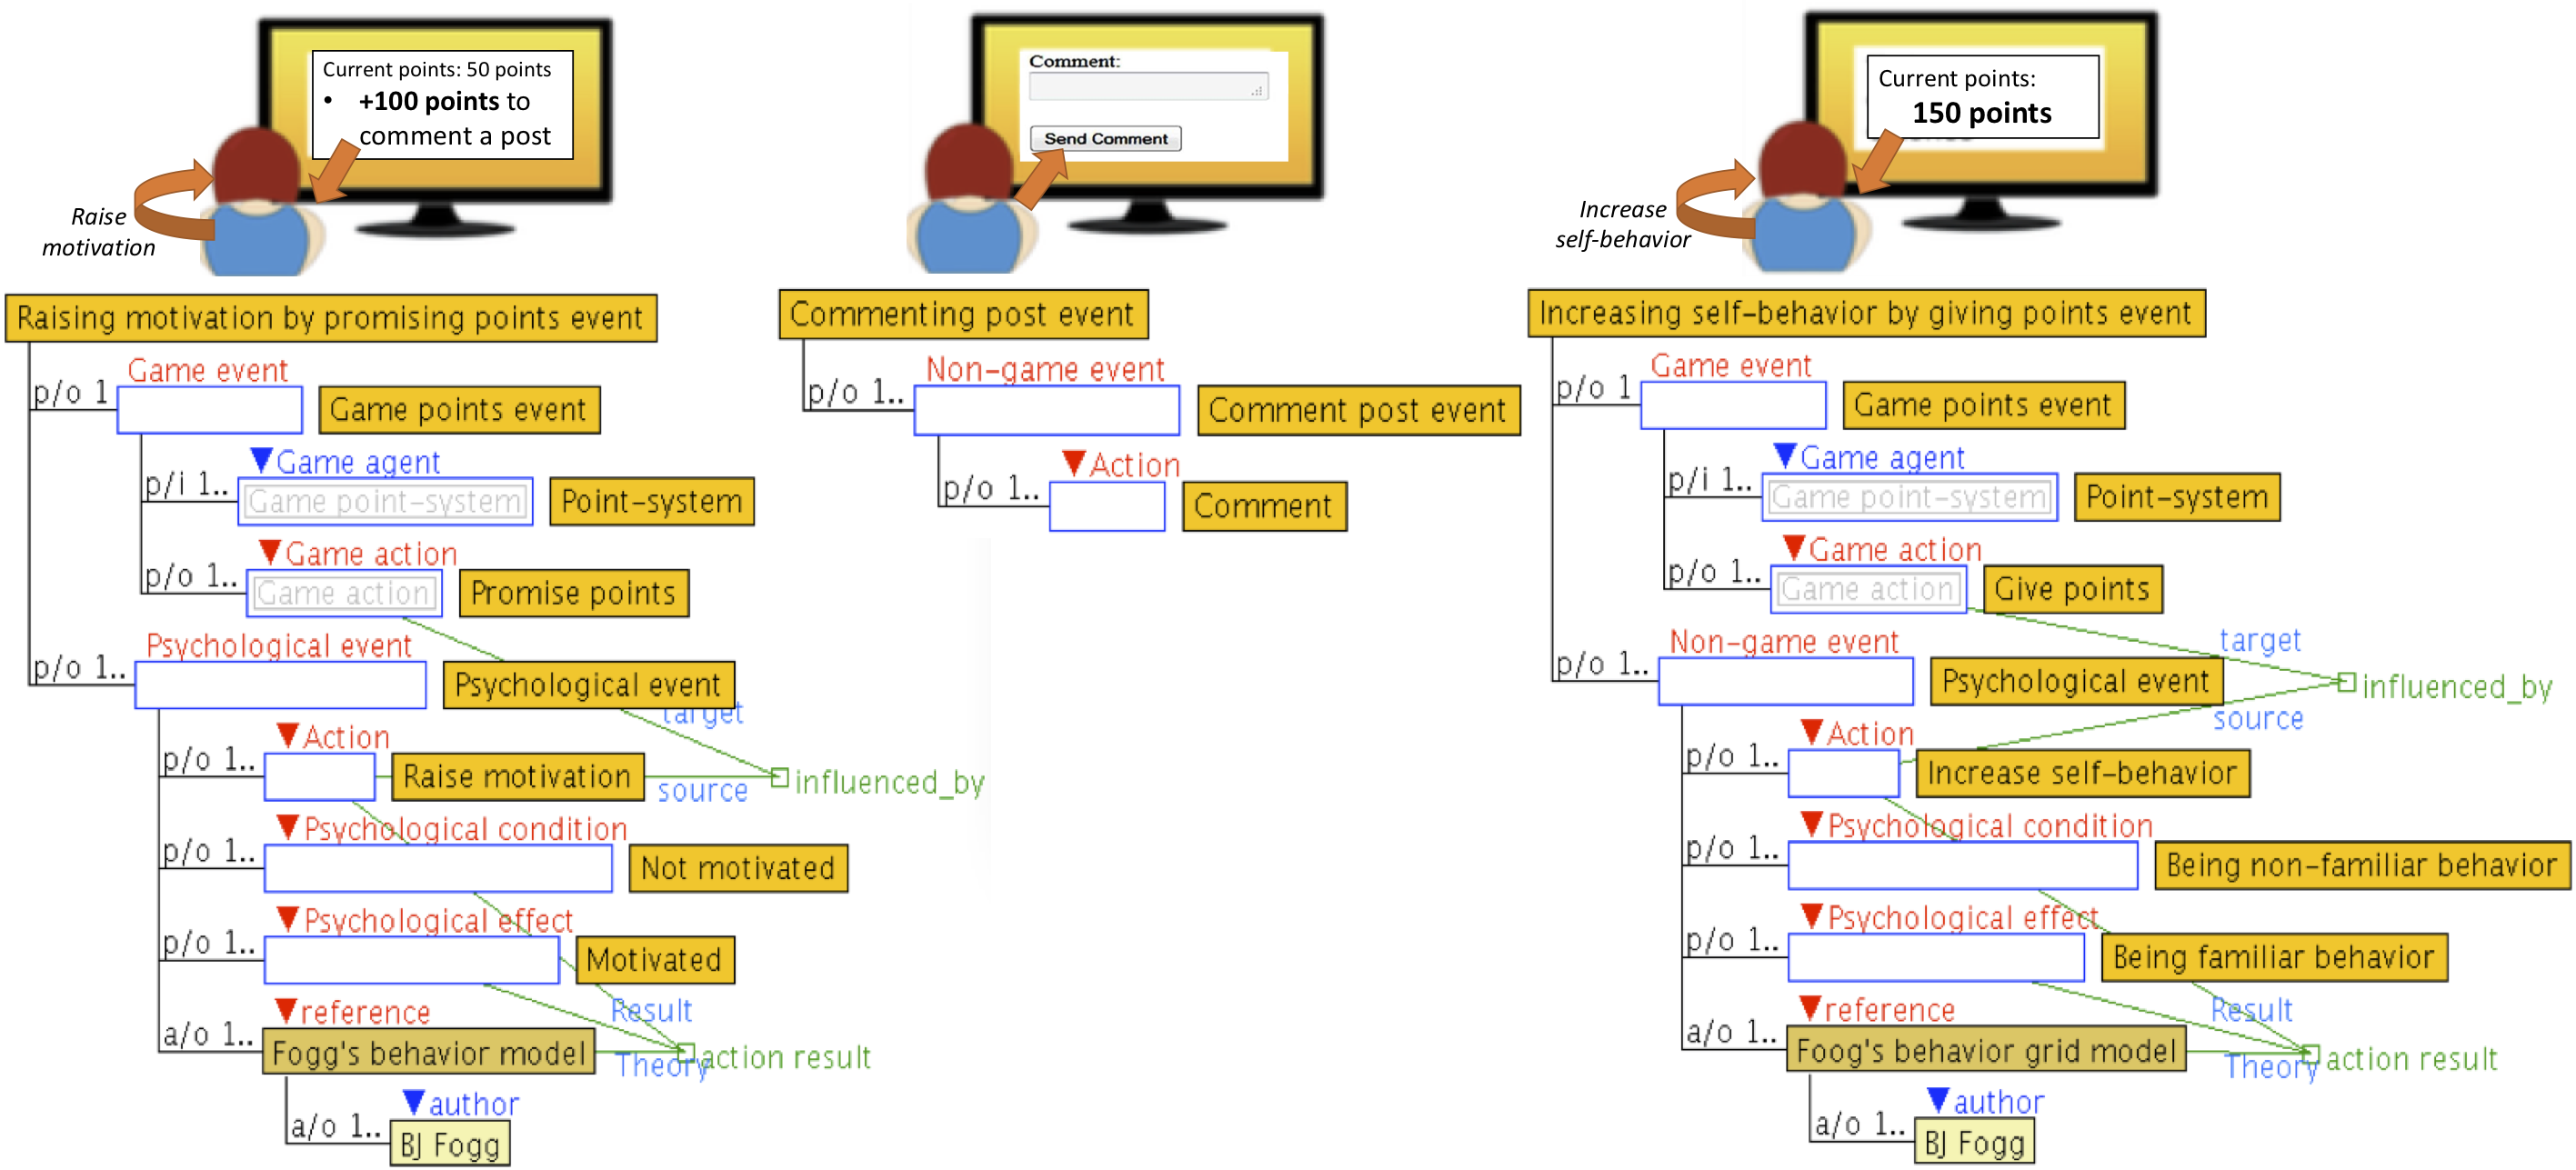
\includegraphics[width=1\textwidth]{images/chap-ontogacles2/ontological-structures-example-persuasive-gameplay-events.png}
 \fautor
\end{figure}







\aspas{\emph{C}} shown ,  for instance, the 


In this interaction, as shown in ontological structure to represent \emph{Gameplay event} (at the top of \autoref{fig:ontological-structures-persuasive-gameplay-event}), the \emph{Game event} 









 Therefore

This interaction represented as the ontological structure shown at the top of \autoref{fig:ontological-structures-persuasive-gameplay-event}



Thus, in the ontological structure to represent a \emph{Gameplay event},  to produce t changes as 

are produced by an \emph{agent} 


Thus,  In the \emph{Game event}, 


As was mentioned before, gameplay of a gamified CL scenario is defined by the way in which the interactions between the participants and the game elements could occur. When a participant interacts with the game elements, the rules defined in the gamified CL scenario process his/her inputs causing changes in the game elements, and these modifications are communicated to the participant. These rules and changes are related to individual motivational goals that must be achieved by the participants, so that each participant has his/her own strategy to interact with the gamified CL scenario to achieve these goals. 


Gameplay event is a prescriptive description of a PGD as a chunk of process between the game elements and the participants of a non-game context being gamified.

In the gamification of CL scenarios, this chuck of process has the purpose to persuade the participants to perform an interaction defined in the sequencing mechanism of CSCL script. 

definition of interactions in this process consists 

Gamification defines a gameplay process to motivate and engage the participants in a non-game process; and the gameplay event is a chunk of this process.

Thus, the gameplay event defines the interactions between the game elements and the participants of non-game process. The relation between game events and non-game events is explicitly represented in the ontology OntoGaCLeS under the concept of Gameplay event. This concept describes, in an explicit way, what happens in the non-game world and the game world when a user performs the processes (actions) defined in the non-game event.


\newpage
\subsection{WAY-knowledge of PGD}
\label{subsec:way-knowledge-of-persuasive-game-design}

 is a prescriptive description of this relation.

\newpage
\subsection{Persuasive Game Design CL Scenario Model}
\label{subsec:persuasive-game-design-cl-scenario-model}






%%%%%%%%%%%%%%%%%%%%%%%%%%%%%%%%%%%%%%%%%%%%%%%%%%
\section[Modeling CL Gameplay Based on Persuasive Game Design]{Modeling Collaborative Learning Gameplay Based on Persuasive Game Design}
\label{sec:modeling-cl-gameplay-persuasive-game-design}


%%%%%%%%%%%%%%%%%%%%%%%%%%%%%%%%%%%%%%%%%%%%%%%%%%
\section[Formalizing an Ontological Model to Apply Gamification as a Persuasive Technology in CL Scenarios]{Formalizing an Ontological Model to Apply Gamification as a Persuasive Technology in Collaborative Learning Scenarios}
\label{sec:formalizing-ontological-model-apply-gamification-persuasive-technology}



 an ontological model to apply gamification as a  employing the persuasive game design strategies defined in the Model-driven persuasive game proposed by \citeonline{Orji2014}.
 
 
%%%%%%%%%%%%%%%%%%%%%%%%%%%%%%%%%%%%%%%%%%%%%%%%%%
\section{Concluding Remarks}
\label{sec:ontogacles2-concluding-remarks} 

 
